\chapter{Dust-to-Gas Ratio and $\alpha_{CO}$}

\section{Minimizing the Scatter in the Dust-to-Gas Ratio}

In order to determine the amount of molecular hydrogen present, we have chosen to use the dust based method to determine the CO-to-H$_2$ conversion factor.  In our analysis we have used the conversion factor $\alpha_{CO}$ which will return the amount of molecular hydrogen present in units of surface density.  Calculating the amount of molecular hydrogen present with this method involves minimizinging the scatter in the dust to gas ratio for a collection of pixels in a region.  The dust-to-gas ratio is calculated using

\begin{equation}\label{eq:dgr}
  \delta_{DGR} = \frac{\Sigma_{dust}}{I_{CO}*\alpha_{CO} + \Sigma_{HI}}
\end{equation}

\noindent where $\delta_{DGR}$ is the ratio of the surface densities of the dust and gas present in the system, $\Sigma_{dust}$ is the surface density of the dust in M$_\odot$ pc$^{-2}$, $I_{CO}$ is the CO intensity in K km s$^{-1}$, $\alpha_{CO}$ is the conversion factor in units of M$_\odot$ pc$^{-2}$ (K km s$^{-1}$)$^{-1}$, and $\Sigma_{HI}$ is the surface density of the atomic hydrogen in M$_\odot$ pc$^{-2}$.  The scatter of the dust-to-gas ratio is determined by finding the standard deviation of the dust-to-gas ratios for the pixels assuming a Gaussian distribution.  

In addition, the atomic hydrogen surface density map had a cut applied to it where any points below 20\% of the maximum surface density were set to zero.  Applying this cut removed all but two of the pixels associated with the nuclear region (region 3 from Figure \ref{fig:regions}).  By removing most of the data, the variation of the scatter in the dust-to-gas ratio with $\alpha_{CO}$ does not show as dramatic an upturn at higher $\alpha_{CO}$ as other regions do.  Therefore region 3 has been omitted from our analysis.

The best fit values for $\delta_{DGR}$ and $\alpha_{CO}$ were determined using the dust surface densities found in Chapter \ref{sed} for both the Planck and the Li and Draine models.  The $\alpha_{CO}$ variable was handled by assigning it a single value over the range of 0.01 to 100 M$_\odot$ pc$^{-2}$ (K km s$^{-1}$)$^{-1}$, and the best-fit $\alpha_{CO}$ was determined by the value resulting in the lowest scatter in the dust-to-gas ratio for the pixels of each region from Figure \ref{fig:regions}.  In addition, a 7$^{th}$ region was added that is the galaxy without the nucleus.  This 7$^{th}$ region was created to accommodate the lack of HI emission in the nucleus of NGC3627.  Once the best $\alpha_{CO}$ is found, the surface density of molecular hydrogen is then determined by scaling the CO intensity by the calculated conversion factor.   Finally, the dust-to-gas ratio is found by dividing the dust surface density by the sum of the HI and H$_2$ surface densities.  

The results using the Planck model with the CO J=1-0 line are shown in Figure \ref{fig:dgr_co10} where the left panel shows the value of the dust-to-gas ratio in each pixel versus the H$_2$ to HI ratio, with the solid red line indicating the mean value for the dust-to-gas ratio, and the dotted lines showing the standard deviation of the dust-to-gas ratio.  The right panels of Figure \ref{fig:dgr_co10} show the scatter in the dust-to-gas ratio as a function of the $\alpha_{CO}$ value adopted.  The numerical values of the dust-to-gas ratio, $\alpha_{CO}$, and H$_2$ surface density using both the Planck and the Li and Draine dust masses are shown in Table \ref{tab:dgr_10t}.  The behavior of the mean dust-to-gas ratio as a function of $\alpha_{CO}$ is shown in Figure \ref{fig:aco_dgr}, and shows that as the conversion factor is increased the amount of gas increases, and with a fixed dust surface density, the dust-to-gas ratio decreases.  The error in the dust-to-gas ratio in Table \ref{tab:dgr_10t} is the same as the minimum scatter found in Figure \ref{fig:dgr_co10}, and the error reported for $\alpha_{CO}$ is half of the spacing between the values used to calculate the minimum scatter.

\begin{figure}%\label{fig:dgr_co10}
  \begin{subfigure}[t]{1\textwidth}
    \centering
    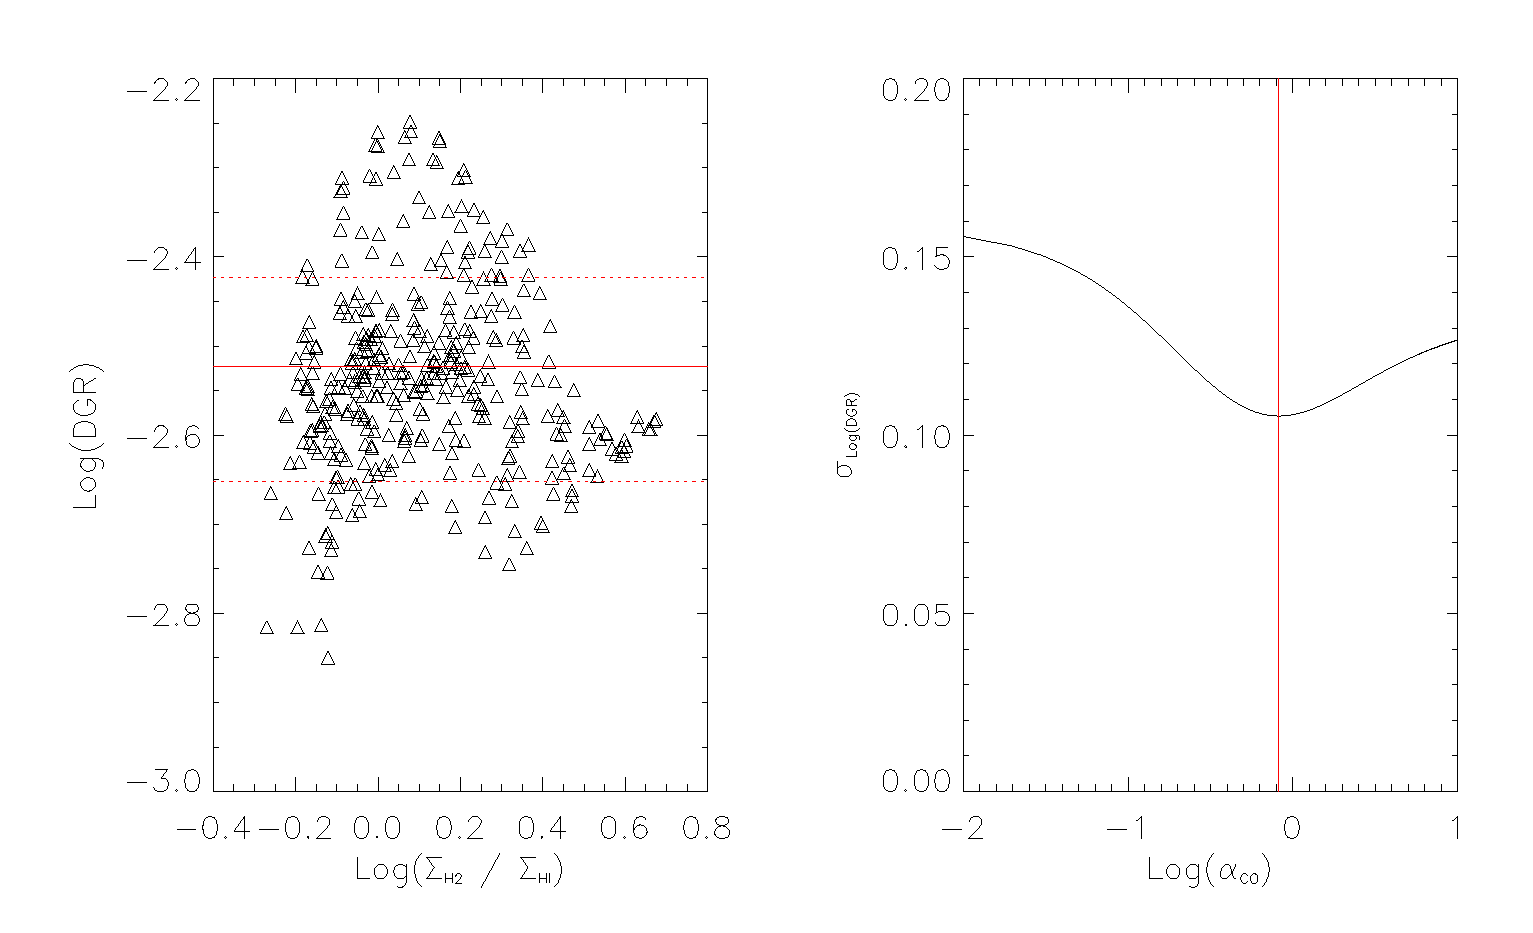
\includegraphics[width=1.\textwidth]{dgr_imgs/region_1_aco_output_10.eps}
    \caption{Region 1}
  \end{subfigure}

  \begin{subfigure}[t]{1\textwidth}
    \centering
    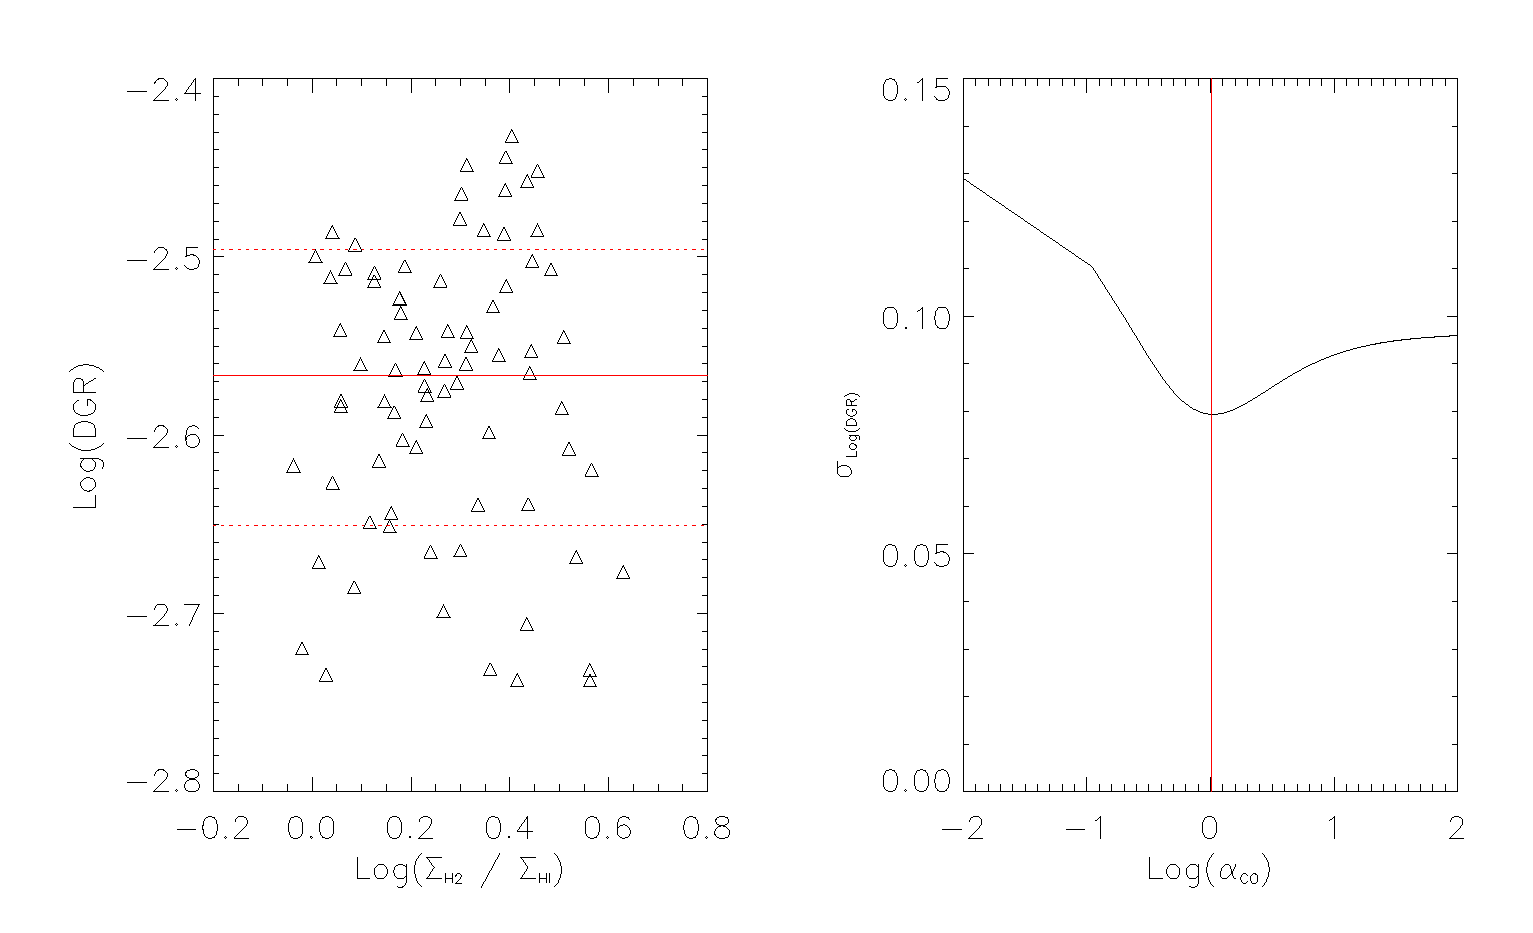
\includegraphics[width=1.\textwidth]{dgr_imgs/region_2_aco_output_10.eps}
    \caption{Region 2}
  \end{subfigure}
   \caption[Dust-to-Gas Ratio Determination Plots for CO J=1-0]{Plots of the dust-to-gas ratio vs the H$_2$ to HI surface density using the best fit $\alpha_{CO}$ (left) and the scatter in the dust-to-gas ratio as a function of $\alpha_{CO}$ (right).  Each parameter was calculated using the CO J=1-0 line and the Planck dust model.}
   \label{fig:dgr_co10}
\end{figure}

\begin{figure}  
  \ContinuedFloat
  \begin{subfigure}[t]{1\textwidth}
    \centering
    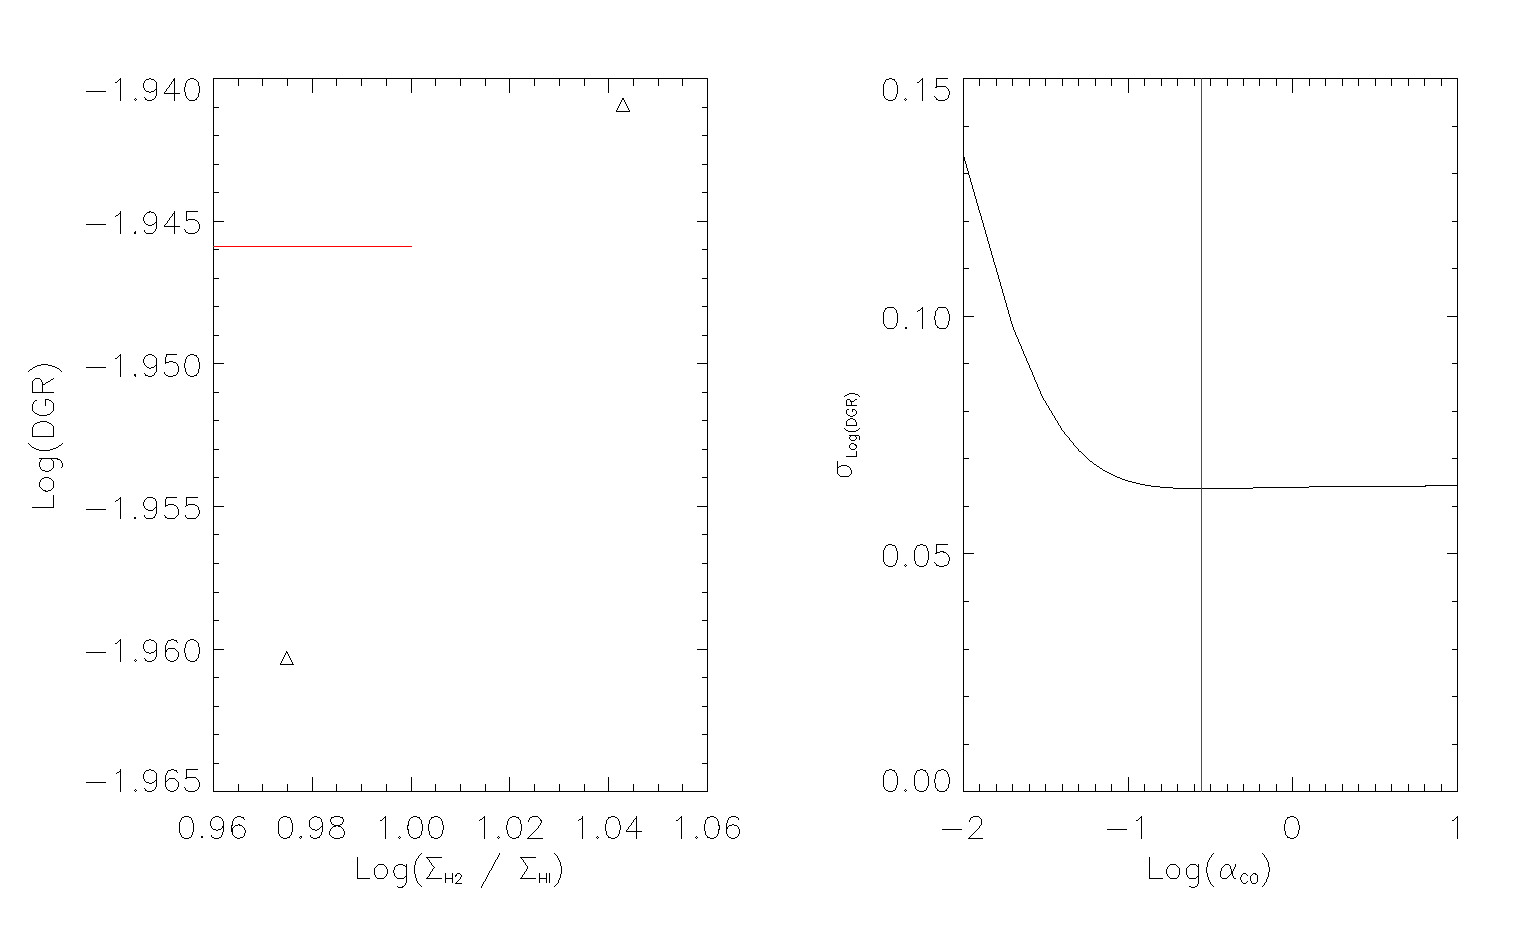
\includegraphics[width=1.\textwidth]{dgr_imgs/region_3_aco_output_10.eps}
    \caption{Region 3}
    \label{fig:dgr_co10_3}
  \end{subfigure}

  \begin{subfigure}[t]{1\textwidth}
    \centering
    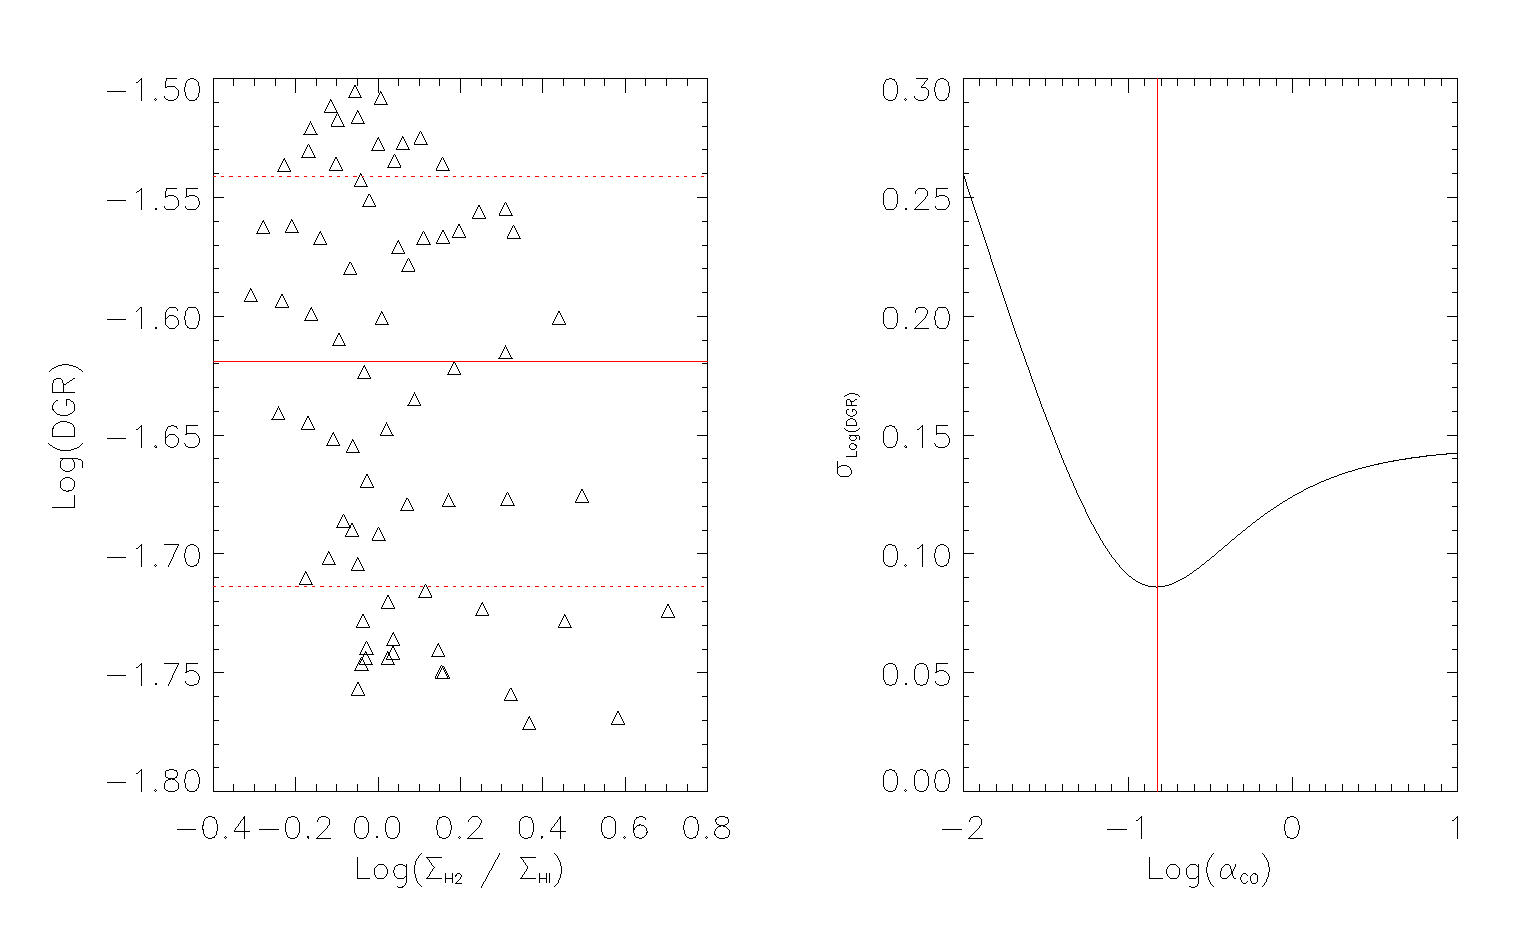
\includegraphics[width=1.\textwidth]{dgr_imgs/region_4_aco_output_10.eps}
    \caption{Region 4}
  \end{subfigure}
   \caption{(continued)}
   \label{fig:dgr_co10}
\end{figure}

\begin{figure}
  \ContinuedFloat
  \begin{subfigure}[t]{1\textwidth}
    \centering
    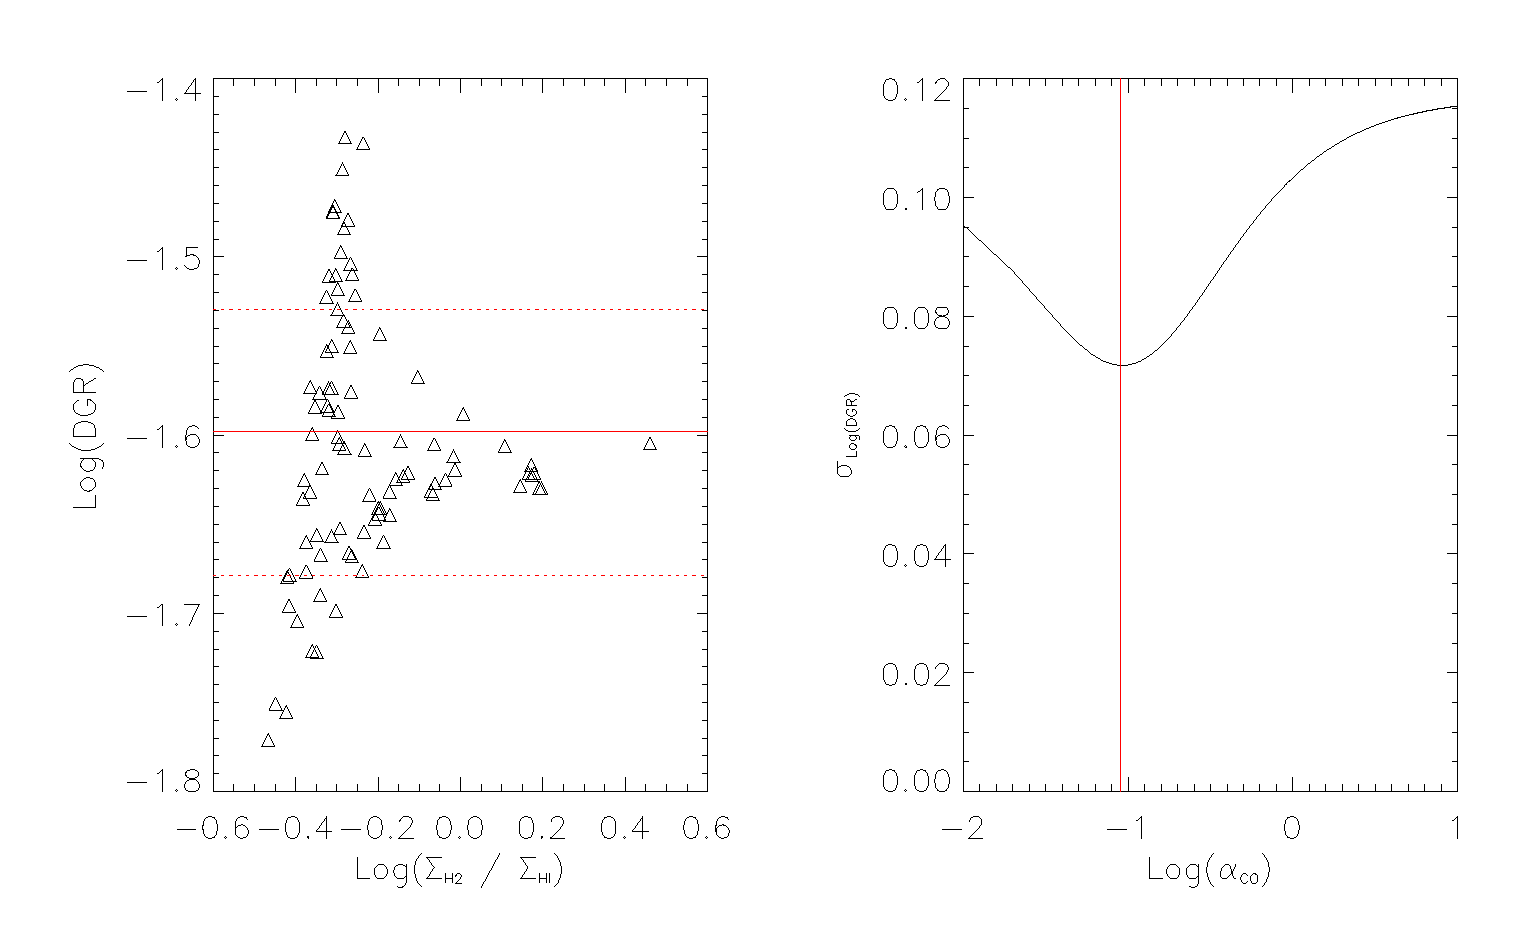
\includegraphics[width=1.\textwidth]{dgr_imgs/region_5_aco_output_10.eps}
    \caption{Region 5}
  \end{subfigure}

  \begin{subfigure}[t]{1\textwidth}
    \centering
    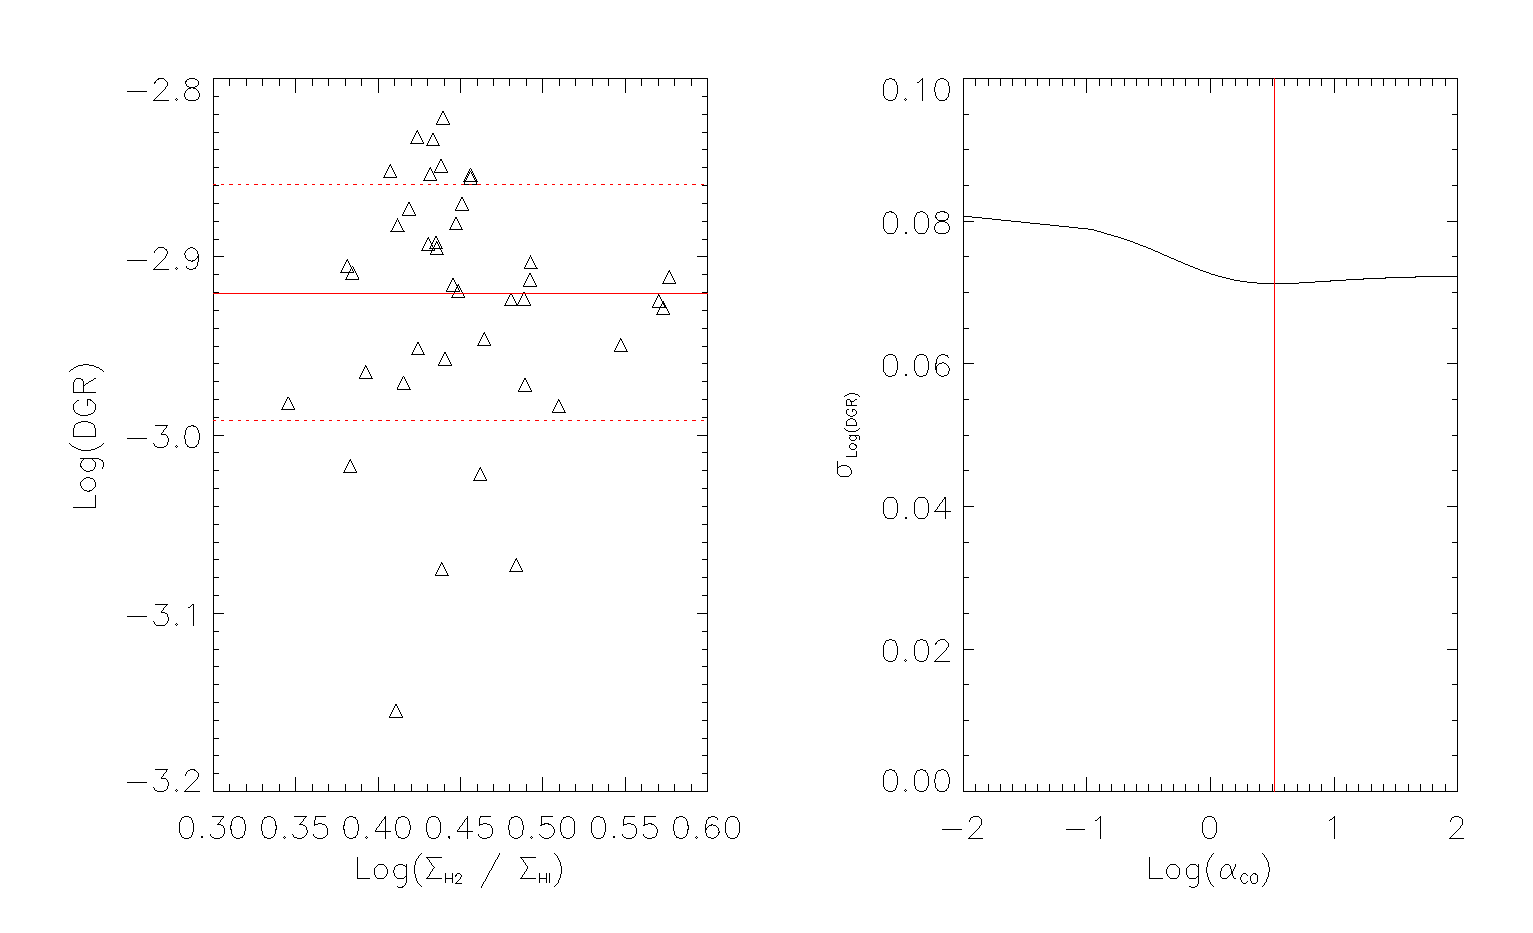
\includegraphics[width=1.\textwidth]{dgr_imgs/region_6_aco_output_10.eps}
    \caption{Region 6}
  \end{subfigure}
   \caption{(continued)}
   \label{fig:dgr_co10}
\end{figure}

\begin{figure}
  \ContinuedFloat
  \begin{subfigure}[t]{1\textwidth}
    \centering
    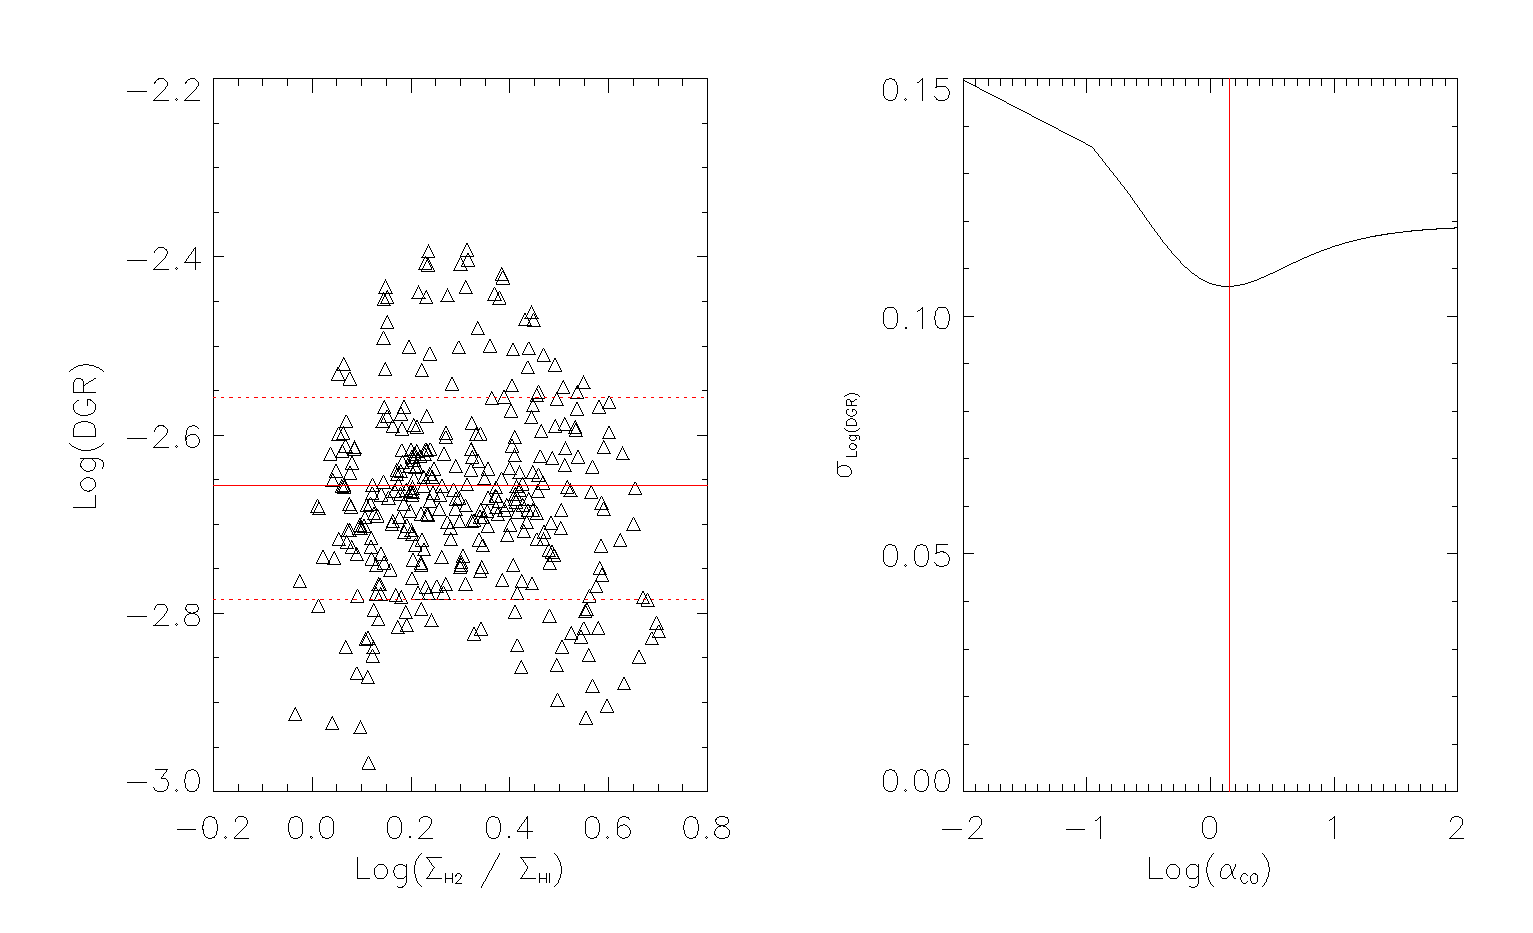
\includegraphics[width=1.\textwidth]{dgr_imgs/region_1-3_aco_output_10.eps}
    \caption{Region 1 Without the Nucleus}
  \end{subfigure}
  \caption{(Continued)}
   \label{fig:dgr_co10}
\end{figure}

\begin{deluxetable}{rccc}
  \tabletypesize{\footnotesize}
  \tablecolumns{4}
  \tablewidth{0pt}
  \tablecaption{Dust-to-gas ratio, $\alpha_{CO}$, and H$_2$ Surface Density using CO J=1-0 as the H$_2$ Tracer\label{tab:dgr_10t}}
  \tablehead{
    \colhead{Opacity Model} &
    \colhead{Dust-to-Gas Ratio} &
    \colhead{$\alpha_{CO}$} &
    \colhead{Average $\Sigma_{H_2}$ per Pixel} \\
    &
    &
    [M$_\odot$ pc$^{-2}$ (K km s$^{-1}$)$^{-1}$] &
    [M$_\odot$ pc$^{-2}$] }
  \startdata
    \sidehead{Region 1}
      Planck &        0.017 $\pm$ 0.004 & 0.230 $\pm$ 0.005 & 4  $\pm$ 3 \\
      Li and Draine & 0.07  $\pm$ 0.02  & 0.230 $\pm$ 0.005 & 4 $\pm$ 3 \\
    \sidehead{Region 2}
      Planck &        0.011 $\pm$ 0.002 & 0.380 $\pm$ 0.005 & 10 $\pm$ 3 \\
      Li and Draine & 0.044 $\pm$ 0.009 & 0.410 $\pm$ 0.005 & 11 $\pm$ 4 \\
%    \sidehead{Region 3}
%      Planck &        0.011 $\pm$ 0.002 & 0.280 $\pm$ 0.005 & 10 $\pm$ 2\\
%      Li and Draine & 0.049 $\pm$ 0.008 & 0.290 $\pm$ 0.005 & 11 $\pm$ 2\\
    \sidehead{Region 4}
      Planck &        0.024 $\pm$ 0.005 & 0.150 $\pm$ 0.005 & 4 $\pm$ 2 \\
      Li and Draine & 0.11  $\pm$ 0.02  & 0.150 $\pm$ 0.005 & 4 $\pm$ 1 \\
    \sidehead{Region 5}
      Planck &        0.03  $\pm$ 0.09  & 0.090 $\pm$ 0.005 & 1.2 $\pm$ 0.6\\
      Li and Draine & 0.11  $\pm$ 0.02  & 0.100 $\pm$ 0.005 & 1.4 $\pm$ 0.6\\
    \sidehead{Region 6}
      Planck &        0.010 $\pm$ 0.001 & 0.590 $\pm$ 0.005 & 6 $\pm$ 1 \\
      Li and Draine & 0.040 $\pm$ 0.006 & 0.610 $\pm$ 0.005 & 6 $\pm$ 1 \\
    \sidehead{No Nucleus}
      Planck &        0.014 $\pm$ 0.004 & 0.300 $\pm$ 0.005 & 5 $\pm$ 3 \\
      Li and Draine & 0.06  $\pm$ 0.02  & 0.310 $\pm$ 0.005 & 5 $\pm$ 3 \\
  \enddata
\end{deluxetable}

\begin{figure}
  \centering
  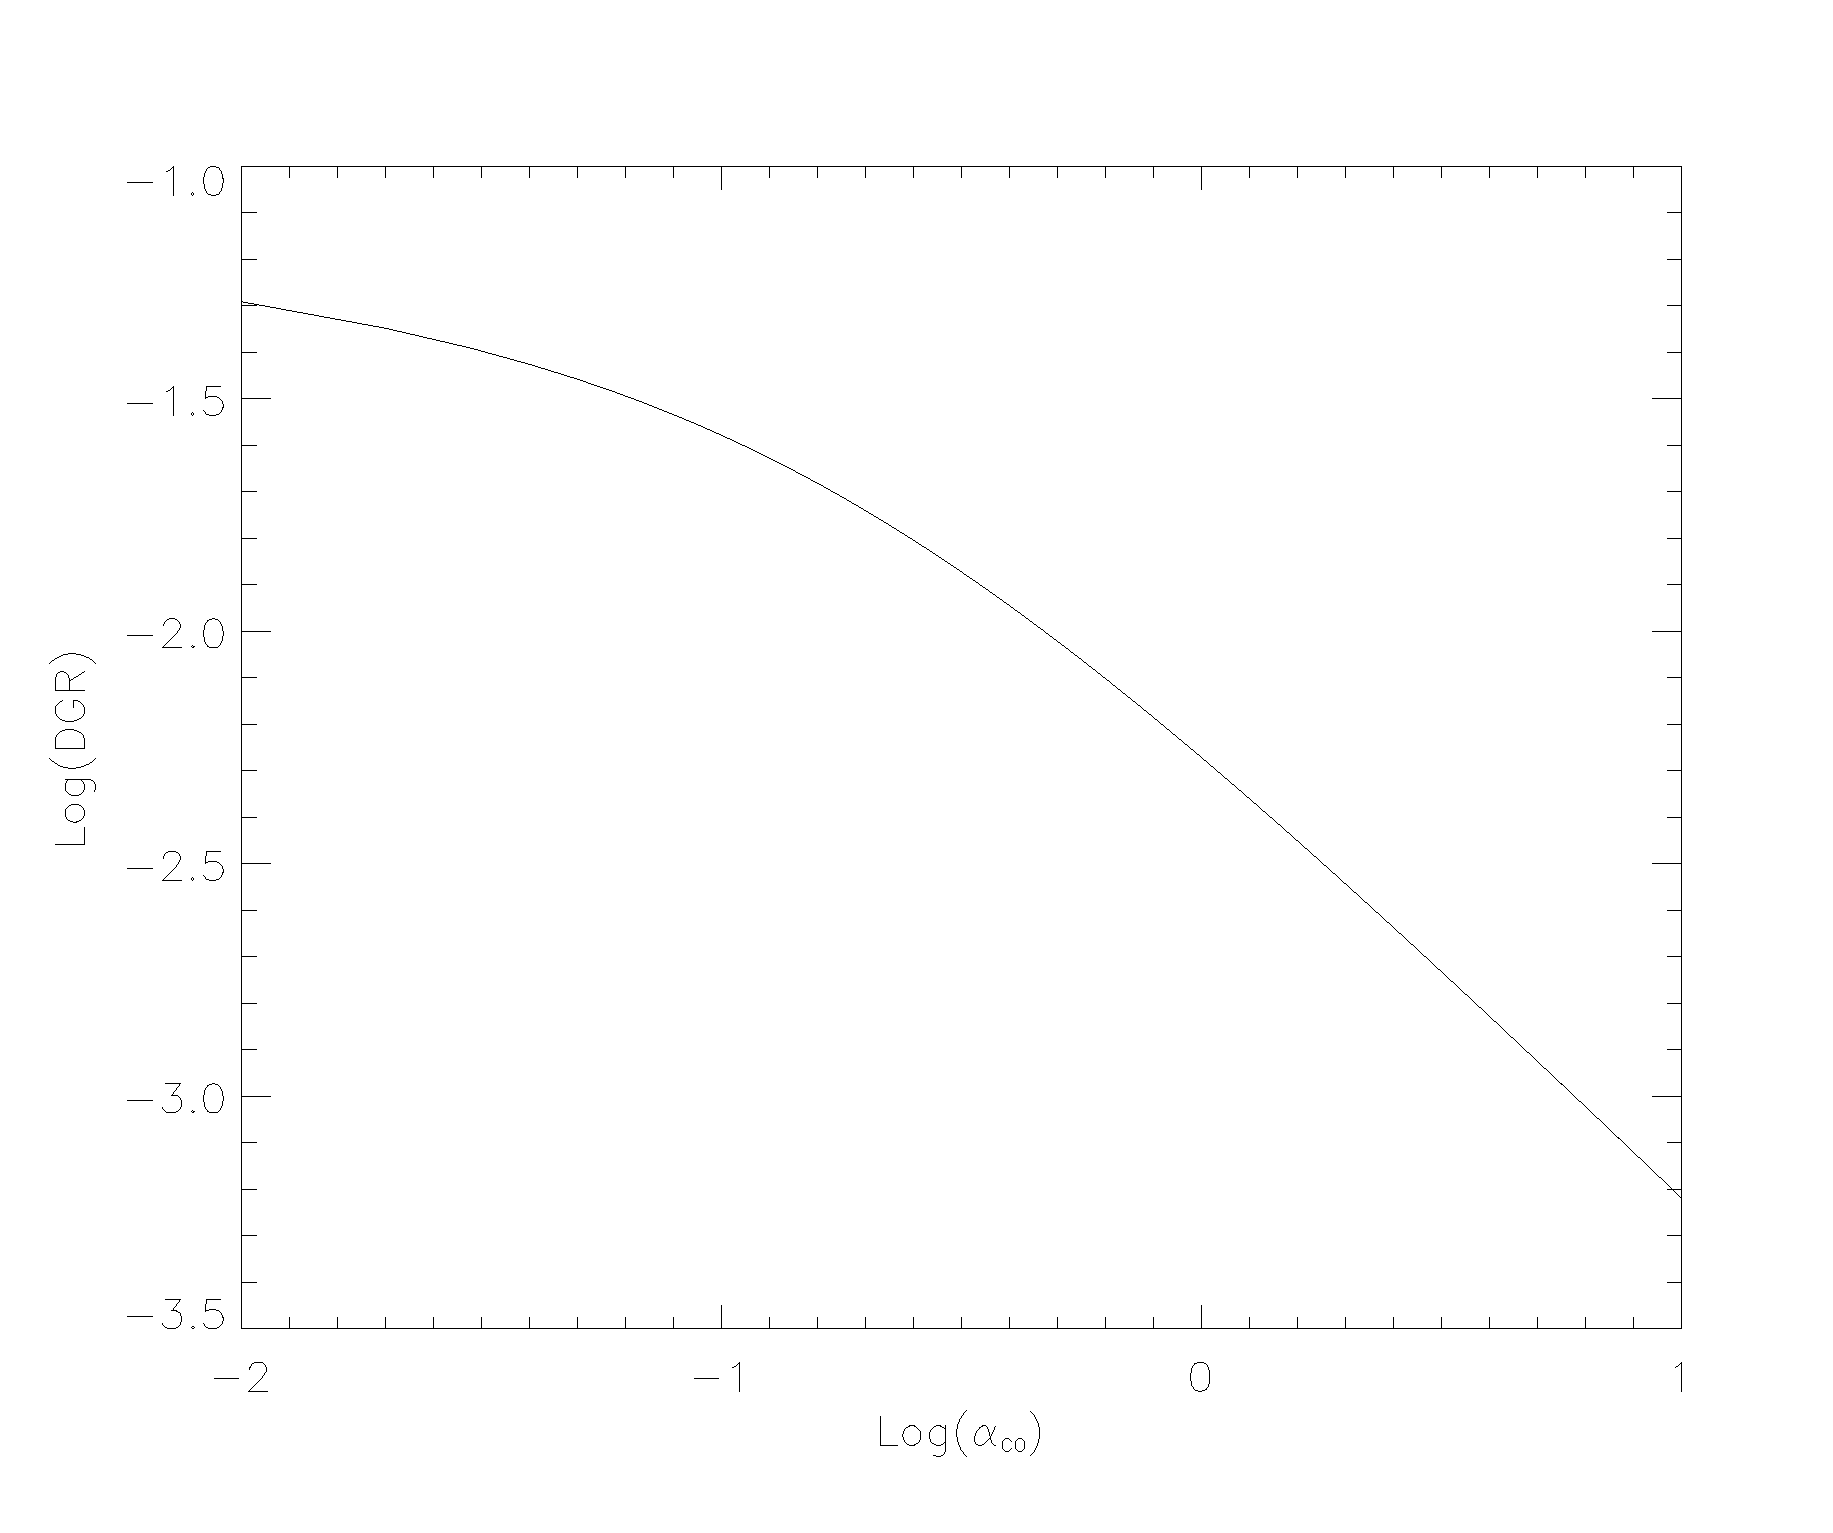
\includegraphics[width=1.\textwidth]{dgr_imgs/region_1-3_aco_dgr.eps}
  \caption[Mean Dust-to-Gas Ratio vs $\alpha_{CO}$]{The dust-to-gas ratio as a function of $\alpha_{CO}$ in region 1 without the nucleus.  The dust model used is the Planck model with CO J=1-0 as the molecular gas tracer.}
  \label{fig:aco_dgr}
\end{figure}

While CO J=1-0 is the standard molecular tracer of H$_2$ \citep{bolatto2013}, these observations are not always available.  When CO J=1-0 data is not available, an alternative rotational transition of CO is used.  For example, \cite{sandstrom2013} used the CO J=2-1 transition, and \cite{warren2010} used the CO J=3-2 transition, where the observations were scaled to the expected intensity of the CO J=1-0 using a ratio of the observed CO transition to the CO J=1-0 transition.  We have measured the CO J=2=1 / J=1-0 line ratio to be 0.39 for the galaxy as a whole, and can examine the effects of using this technique to approximate the CO J=1-0 transition in this method.  The results for the dust-to-gas ratio, $\alpha_{CO}$, and H$_2$ surface density are shown using CO J=2-1 in Table \ref{tab:dgr_21}.

\begin{deluxetable}{rccc}
  \tabletypesize{\footnotesize}
  \tablecolumns{4}
  \tablewidth{0pt}
  \tablecaption{Dust-to-gas ratio, $\alpha_{CO}$, and H$_2$ Surface Density using CO J=2-1 as the H$_2$ Tracer\label{tab:dgr_21}}
  \tablehead{
    \colhead{Opacity Model} &
    \colhead{Dust-to-Gas Ratio} &
    \colhead{$\alpha_{CO}$} &
    \colhead{Average $\Sigma_{H_2}$ per Pixel} \\
    &
    &
    [M$_\odot$ pc$^{-2}$ (K km s$^{-1}$)$^{-1}$] &
    [M$_\odot$ pc$^{-2}$] }
  \startdata
    \sidehead{Region 1}
      Planck &        0.01   $\pm$ 0.01  & 0.390 $\pm$ 0.005 & 8  $\pm$ 5 \\
      Li and Draine & 0.048  $\pm$ 0.01  & 0.410 $\pm$ 0.005 & 8  $\pm$ 5 \\
    \sidehead{Region 2} 
      Planck &        0.0128 $\pm$ 0.004 & 0.310 $\pm$ 0.005 & 8  $\pm$ 3 \\
      Li and Draine & 0.054  $\pm$ 0.003 & 0.330 $\pm$ 0.005 & 8  $\pm$ 3 \\
%    \sidehead{Region 3}
%      Planck &        0.014  $\pm$ 0.009 & 0.270 $\pm$ 0.005 & 9  $\pm$ 2 \\
%      Li and Draine & 0.037   $\pm$ 0.02 & 0.280 $\pm$ 0.005 & 9  $\pm$ 3 \\
    \sidehead{Region 4}
      Planck &        0.0085 $\pm$ 0.004 & 0.520 $\pm$ 0.005 & 15  $\pm$ 1 \\
      Li and Draine & 0.037  $\pm$ 0.005 & 0.540 $\pm$ 0.005 & 16  $\pm$ 6 \\
    \sidehead{Region 5}
      Planck &        0.013  $\pm$ 0.008 & 0.340 $\pm$ 0.005 & 4  $\pm$ 1 \\
      Li and Draine & 0.054  $\pm$ 0.008 & 0.360 $\pm$ 0.005 & 5  $\pm$ 2 \\
    \sidehead{Region 6}
      Planck &        0.0108 $\pm$ 0.004 & 0.450 $\pm$ 0.005 & 5  $\pm$ 1 \\
      Li and Draine & 0.037  $\pm$ 0.004 & 0.460 $\pm$ 0.005 & 5  $\pm$ 2 \\
    \sidehead{No Nucleus}
      Planck &        0.009  $\pm$ 0.007 & 0.550 $\pm$ 0.005 & 10 $\pm$ 6 \\
      Li and Draine & 0.034  $\pm$ 0.008 & 0.580 $\pm$ 0.005 & 10 $\pm$ 6 \\
  \enddata
\end{deluxetable}

\section{Effects of the Dust Model and CO Treatment}

The effects of the dust model (Planck vs Li and Draine) are mainly seen in the dust-to-gas ratio for the CO J=1-0 emission.  Since the major difference in the two models was the resulting dust mass, it is reasonable that the Li and Draine model produces larger dust-to-gas ratios.  The values of $\alpha_{CO}$ derived from the two dust models agree within uncertainty and the overall molecular gas surface densities all agree within error for each region for the two dust models.  The same trend is seen when scaling the CO J=2-1 emission, where the dust-to-gas ratio of the Planck model is also smaller than the Li and Draine model.  %However, for the $\alpha_{CO}$ values, the galaxy as a whole and regions 4 and 5 also show a larger $\alpha_{CO}$ which increases the average surface density of those regions.
  
  The difference in using either the CO J=1-0 or CO J=2-1 as the molecular hydrogen tracer is seen in the value of $\alpha_{CO}$.  Using the CO J=2-1 emission with a 2-1/1-0 ratio applied, the conversion factor is significantly increased in regions 4 and 5, while the conversion factor iss decreased in regions 2 and 6.  The increase in regions 4 and 5 is large enough to increase the conversion factor for the galaxy as a whole despite the decrease in regions 2 and 6.  Despite the change in $\alpha_{CO}$ values in each region, we still see the same masses for all of the regions except for regions 4 and 5.  The change in H$_2$ surface densities are due to the behavior of the 2-1/1-0 ratio in these regions.  Region 5 displays a large gradient in the 2-1/1-0 ratio from north to south along the spiral arm, and the factor of 4 change in region 4 is due to the entire region's 2-1/1-0 ratio being nearly double the mean value of the galaxy. 
  
The difference in $\alpha_{CO}$ between the CO J=1-0 emission and the converted CO J=2-1 emission raises the question of which value we should trust.  The answer lies primarily in whether we are concerned with the dense or diffuse molecular ISM.  If we are interested in the diffuse molecular ISM such as the outer regions of a GMC, \cite{wilson1990} showed in M33 that over half of the CO J=1-0 emission is due to diffuse gas, so using this transition would be ideal.  If the dense molecular ISM is being examined such as the inner regions of a GMC, then the CO J=2-1 emission would be more appropriate to determine the H$_2$ abundance.  Since we are not able to resolve individual GMCs and are interested in the overall molecular ISM of NGC3627, both play a role in understanding the abundance of H$_2$ in the system.

\section{Comparison of Results with Previous Work}

If NGC3627 were to have Milky Way like values for $\alpha_{CO}$, we would expect $\alpha_{CO}\approx$4 \citep{sandstrom2013}.  However, the $\alpha_{CO}$ values calculated using the the CO J=2-1 emission suggest NGC3627 is similar to U/LIRG type galaxies whose $\alpha_{CO}$ range is more like 0.3 - 1.3 M$_\odot$ pc$^{-2}$ (K km s$^{-1}$)$^{-1}$ \citep{downes1998}.  The results using the CO J=1-0 emission fall below even the U/LIRG range.  Even our smallest dust-to-gas ratio lies above the typical values found in late type galaxies of 0.005 - 0.01 \citep{smith2012}.  If we compare our Li and Draine results to values recently calculated using the same method by \cite{sandstrom2013}, we find that our conversion factor is much lower than their average for NGC3627 of 1.2 M$_\odot$ pc$^{-2}$ (K km s$^{-1}$)$^{-1}$, and our dust-to-gas ratio is much larger than their average of $\approx$0.017.  

The low $\alpha_{CO}$ and high dust-to-gas ratios are likely due to the filtering process applied to our data ($\S$\ref{ancillary}), in particular, the amount of the HI surface density removed by the filtering.  If the HI emission is small, the product of I$_{CO}\alpha_{CO}$ will dominate the denominator of equation \ref{eq:dgr} essentially removing the $\Sigma_{HI}$ term.  The effect of this would result in 

\begin{equation}\label{dgr:degen}
  \delta_{dgr}\alpha_{CO} = \frac{\Sigma_{dust}}{I_{CO}}
\end{equation}

\noindent where the degeneracy between $\delta_{dgr}$ and $\alpha_{CO}$ is apparent.  By removing a significant portion of the HI surface density we have weakened the constraint of the method, and strengthened the possibility for degeneracy.

As a crude test, we used the unfiltered gas data with the filtered Li and Draine dust surface densities to establish comparable values with the results reported by \cite{sandstrom2013}.  This process gives the results shown in Table \ref{tab:no_filt} and a plot similar to Figure \ref{fig:dgr_co10} for region 1 with the nucleus removed is shown in Figure \ref{fig:filt_dgr}.  The unfiltered mean dust-to-gas ratio is shown a function of $\alpha_{CO}$ in Figure \ref{fig:filt_aco_dgr} where the increase in the HI surface density has introduced a plateau at low values for $\alpha_{CO}$.  Removing the filtering has increased the CO J=2-1 results to be in reasonable agreement with the values from \cite{sandstrom2013} over region 1.  The lower dust-to-gas ratios are primarily attributed to the spatial filtering that has occurred, but can also be linked to how the dust mass was calculated.  Using the method we used to determine the dust mass by fitting a single blackbody fit over the cold component can lead to a dust mass nearly a factor of two larger compared to the approach taken by \cite{sandstrom2013} of using the entire infrared spectrum \citep{dale2012}.

\begin{deluxetable}{cccc}
  \tabletypesize{\footnotesize}
  \tablecolumns{4}
  \tablewidth{0pt}
  \tablecaption{CO Transition, $\alpha_{CO}$, and H$_2$ Surface Density using the Li and Draine dust model with No Spatial Filtering of CO or HI \label{tab:no_filt}}
  \tablehead{
    \colhead{Region} &
    \colhead{Dust-to-Gas Ratio} &
    \colhead{$\alpha_{CO}$} &
    \colhead{Average $\Sigma_{H_2}$ per Pixel} \\
    &
    &
    [M$_\odot$ pc$^{-2}$ (K km s$^{-1}$)$^{-1}$] &
    [M$_\odot$ pc$^{-2}$] }
  \startdata
    \sidehead{Region 1}
      J=1-0 & 0.013  $\pm$ 0.003  & 0.880 $\pm$ 0.005 & 21 $\pm$ 10  \\
      J=2-1 & 0.010  $\pm$ 0.001  & 1.520 $\pm$ 0.005 & 32 $\pm$ 18 \\
    \sidehead{Region 2}
      J=1-0 & 0.011  $\pm$ 0.002  & 1.130 $\pm$ 0.005 & 33 $\pm$ 11 \\
      J=2-1 & 0.0106 $\pm$ 0.0009 & 1.360 $\pm$ 0.005 & 36 $\pm$ 15 \\
%    \sidehead{Region 3}
%      J=1-0 & 0.0032 $\pm$ 0.0003 & 0.580 $\pm$ 0.005 & 25 $\pm$ 5  \\
%      J=2-1 & 0.0040 $\pm$ 0.0002 & 0.520 $\pm$ 0.005 & 18 $\pm$ 5  \\
    \sidehead{Region 4}
      J=1-0 & 0.035  $\pm$ 0.006  & 0.130 $\pm$ 0.005 & 4  $\pm$ 1  \\
      J=2-1 & 0.013  $\pm$ 0.001  & 1.170 $\pm$ 0.005 & 36 $\pm$ 12 \\
    \sidehead{Region 5}
      J=1-0 & 0.013  $\pm$ 0.001  & 0.720 $\pm$ 0.005 & 14 $\pm$ 5  \\
      J=2-1 & 0.009  $\pm$ 0.0009 & 1.98  $\pm$ 0.005 & 28 $\pm$ 9  \\
    \sidehead{Region 6}
      J=1-0 & 0.0050 $\pm$ 0.0007 & 3.780 $\pm$ 0.005 & 53 $\pm$ 8  \\
      J=2-1 & 0.0065 $\pm$ 0.0007 & 3.090 $\pm$ 0.005 & 35 $\pm$ 10 \\
    \sidehead{No Nucleus}
      J=1-0 & 0.009  $\pm$ 0.002  & 1.470 $\pm$ 0.005 & 32 $\pm$ 14 \\
      J=2-1 & 0.0076 $\pm$ 0.0009 & 2.260 $\pm$ 0.005 & 43 $\pm$ 25 \\
  \enddata
\end{deluxetable}
 
 \begin{figure}
   \centering
   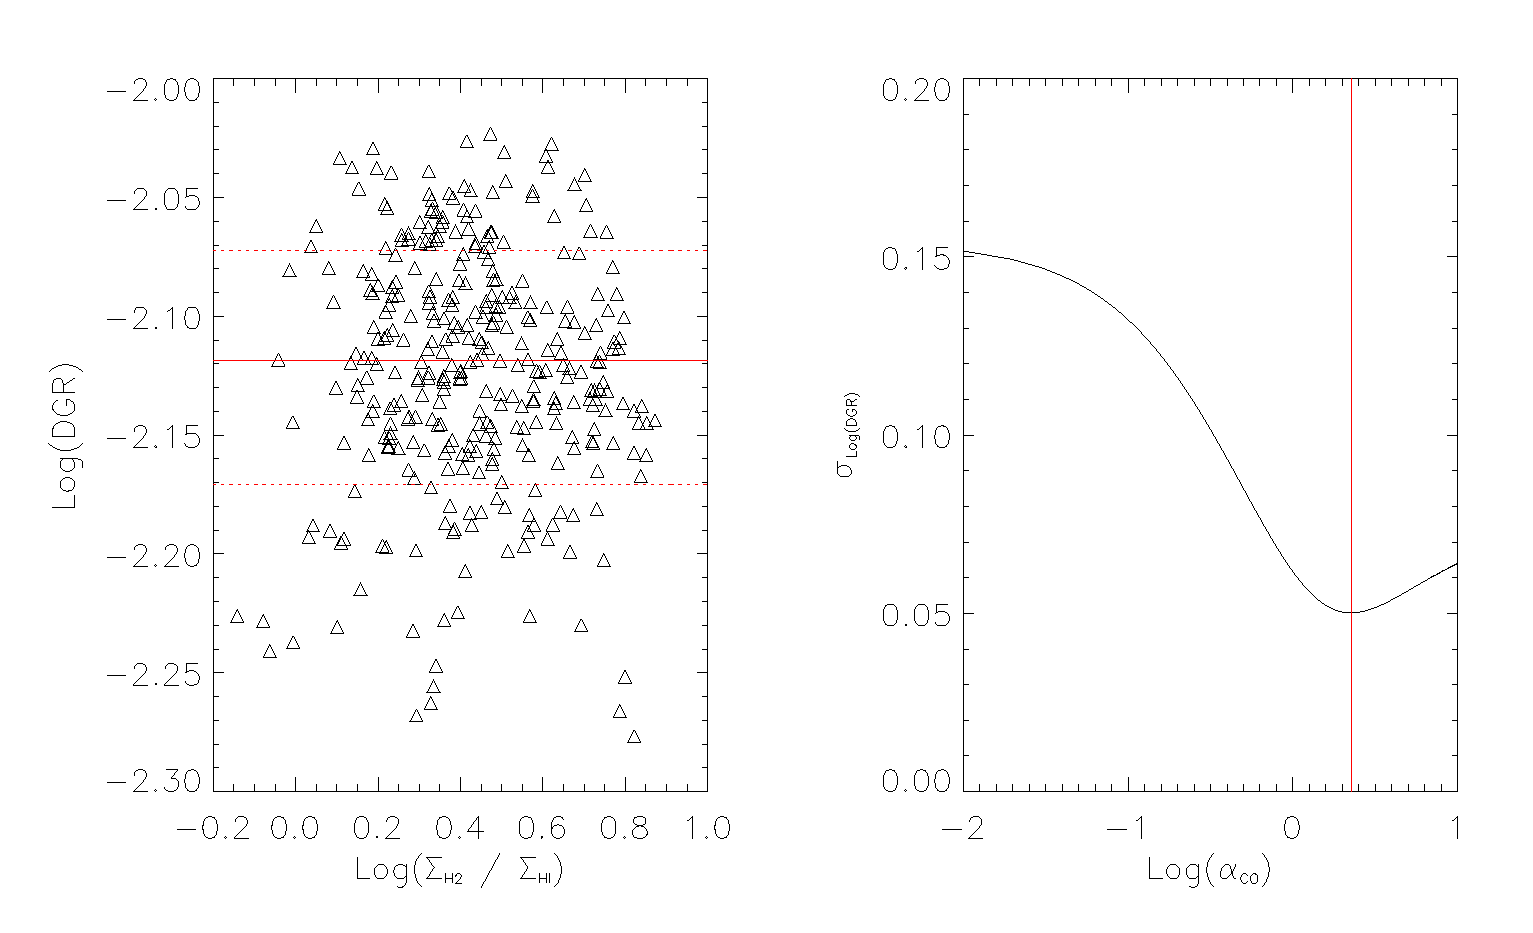
\includegraphics[width=1.\textwidth]{dgr_imgs/region_1-3_aco_output_21_no_filt.eps}
   \caption[Unfiltered Dust-to-Gas Ratio Determination Plots for CO J=2-1]{Plots of the dust-to-gas ratio vs the H$_2$ to HI surface densities using the best fit $\alpha_{CO}$ (left) and the scatter in the dust-to-gas ratio as a function of $\alpha_{CO}$ (right).  The plots were made using the Li and Draine dust model with the CO J=2-1 molecular tracer with the extended emission in the HI and CO J=2-1 data.}
   \label{fig:filt_dgr}
\end{figure}
 
 \begin{figure}
   \centering
   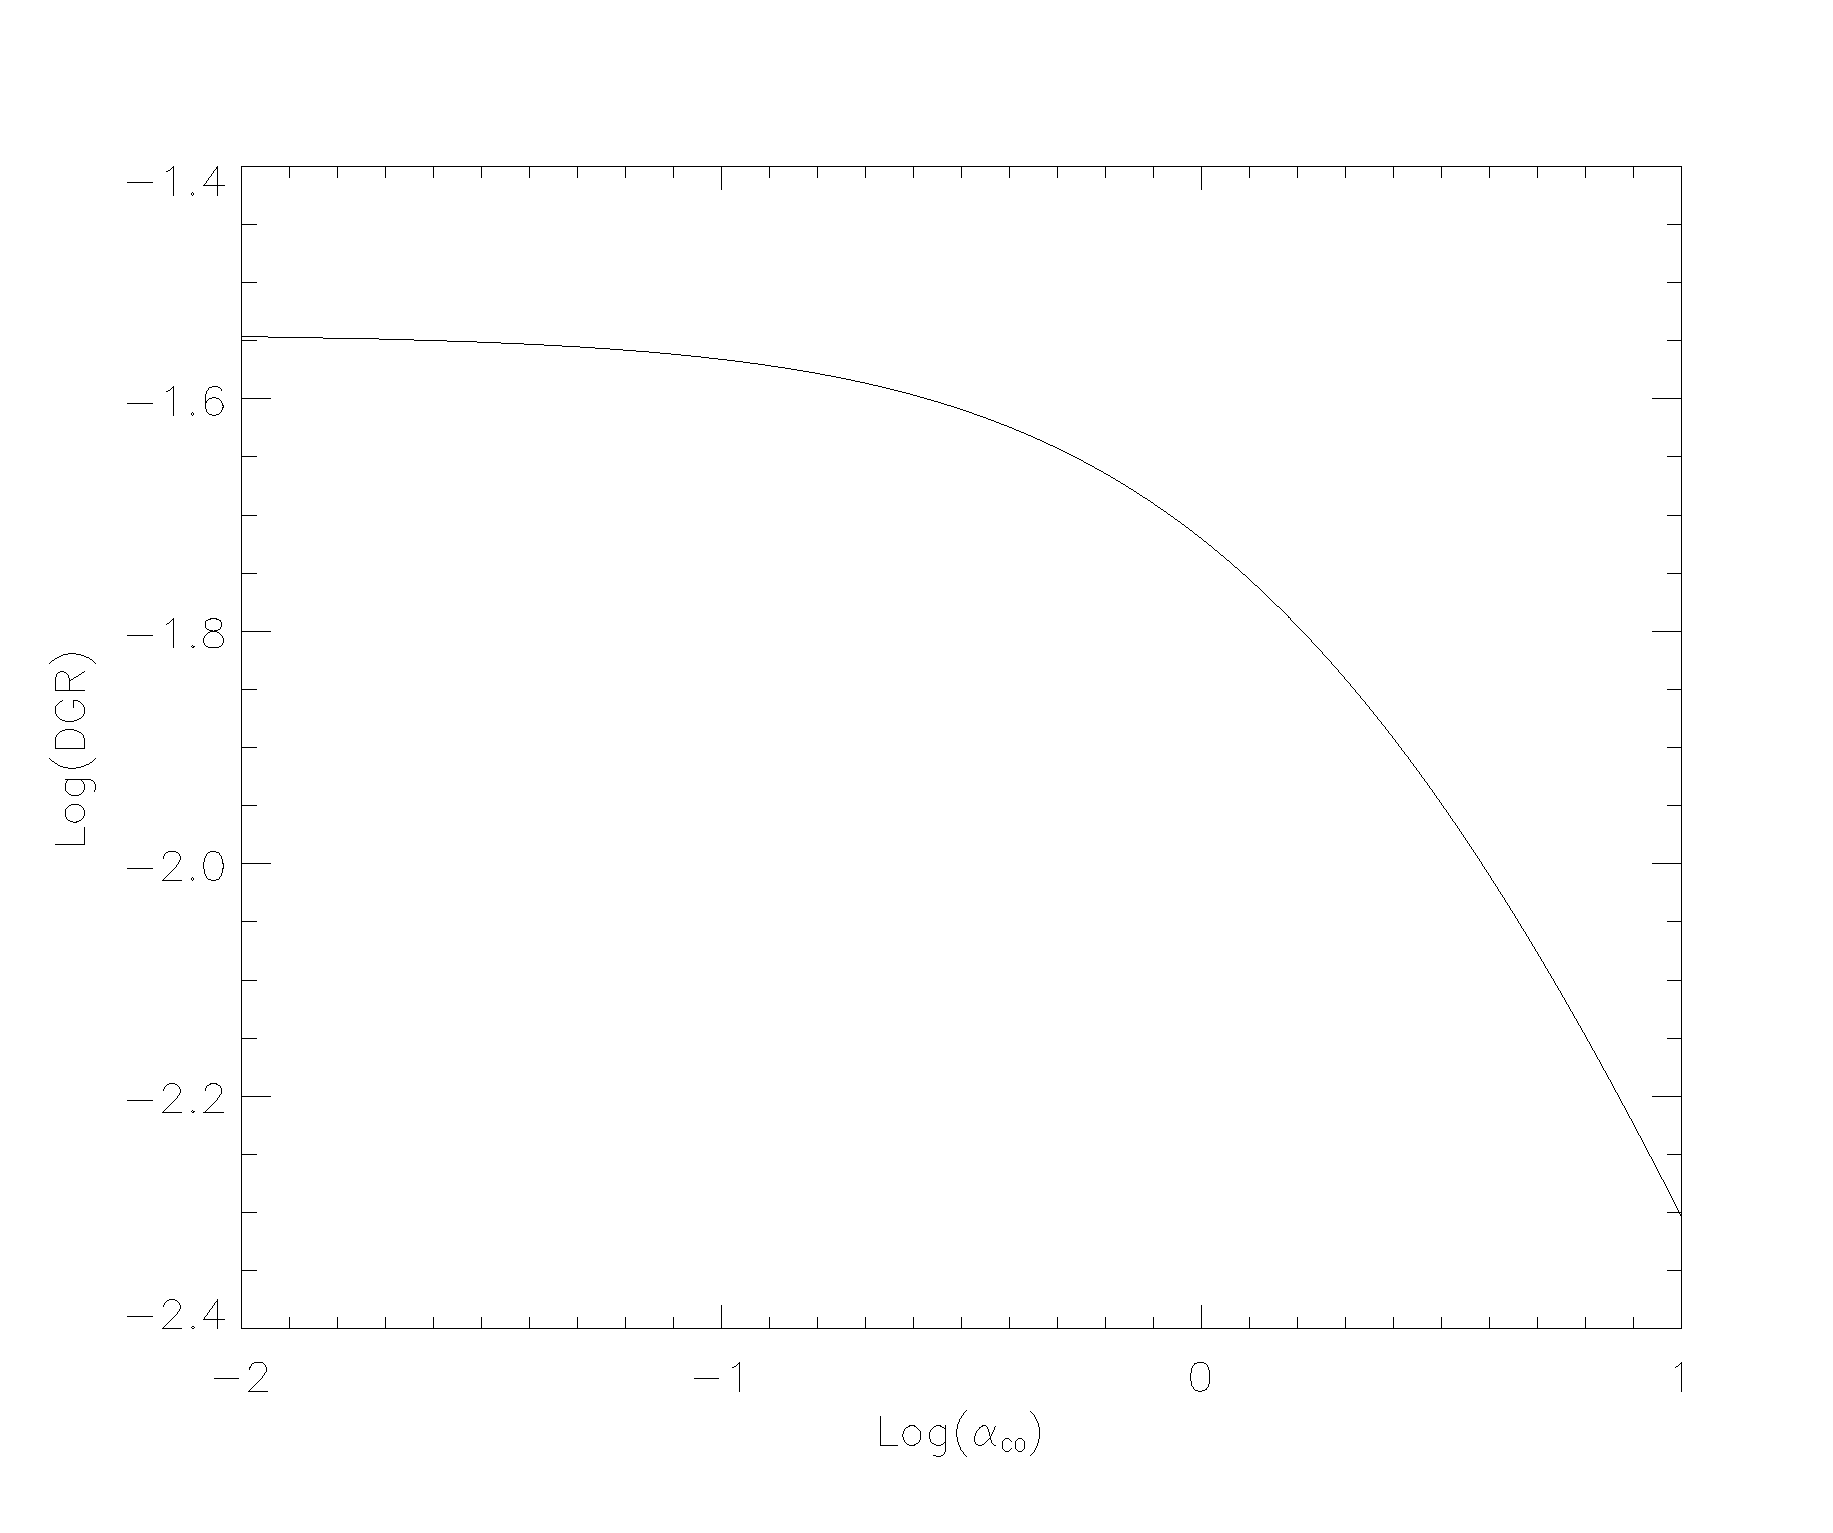
\includegraphics[width=1.\textwidth]{dgr_imgs/region_1-3_aco_dgr_nf.eps}
   \caption[Mean Dust-to-Gas Ratio vs $\alpha_{CO}$ Without Extended Emission Filtering]{The mean dust-to-gas ratio as a function of $\alpha_{CO}$ in region 1 with the nucleus removed using the Li and Draine dust model and the CO J=2-1 emission as the molecular tracer without any extended emission filtering in the HI or CO J=2-1 data.} 
    \label{fig:filt_aco_dgr}
\end{figure}
 
\section{Caveats Due to Uncertainty Estimation}

The values for the uncertainty associated with our best fit $\alpha_{CO}$ come from the step size used when calculating the minimum dust-to-gas ratio scatter.  Comparing region 1 and the region without the nucleus, we would expect the results from the fitting to be the same since the difference is only two points.  In Tables \ref{tab:dgr_10t} and \ref{tab:dgr_21}, we see that excluding these two points did not change the dust-to-gas ratio significantly, but did lead to $\alpha_{CO}$ values that differed by 0.07-0.17 M$_\odot$ pc$^{2-}$ (K km s$^{-1}$)$^{-1}$ which is greater than our reported uncertainty in $\alpha_{CO}$.  The change in $\alpha_{CO}$ over these two regions suggests that we have underestimated the uncertainty in this parameter.  Furthermore, if we adopt the difference of 0.07 as our uncertainty in $\alpha_{CO}$ and convert it to its log space equivalent of 0.13, we can apply this as a horizontal error bar in Figure \ref{fig:dgr_co10}.  If our error bars overlap the portion of the plot to the right of the $\alpha_{CO}$ minimum where the scatter begins to converge to a single value, then the fitted $\alpha_{CO}$ represents more of a minimum value of $\alpha_{CO}$ for the system rather than the actual value.